\section{Introduction}

\begin{frame}{How is cancer usually treated?}
      \begin{figure}[h]
        \centering
        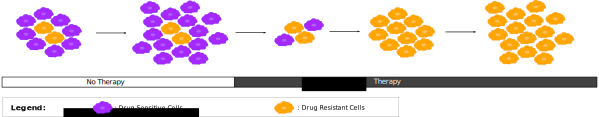
\includegraphics[width=\textwidth]{compe_release}
        \caption{Competitive release under SOC\footnotemark[1]}
      \end{figure}
      \begin{itemize}
        \item<1-> Conventional therapy aims to reduce tumour burden \cite{Frei}
        \item<2-> SOC\footnotemark[1]: Drugs applied at MTD\footnotemark[2]
        \item<3-> Cells have heterogeneous sensitivity $\rightarrow$ without therapy - sensitive keep resistant in check
        \item<4-> MTD\footnotemark[2] eliminates sensitive $\rightarrow$ resistant tumour doesn't respond to therapy \cite{Scott}
      \end{itemize}
      \footnotetext[1]{SOC: Standard-Of-Care}
      \footnotetext[2]{MTD: Maximum Tolerated Dose}
\end{frame}

\begin{frame}{How to avoid competitive release?}
  \begin{figure}[h]
    \centering
    \includegraphics[width=\textwidth]{at}
    \caption{Control under AT\footnotemark[1]}
  \end{figure}
  \begin{itemize}
    \item<1-> AT\footnotemark[1]: apply drugs at lower, fluctuating doses \cite{Gatenby}
    \item<2-> During drug holiday $\rightarrow$ sensitive compete with resistant
    \item<3-> AT\footnotemark[1] outcome depends on competition
  \end{itemize}
  \footnotetext[1]{AT: Adaptive Therapy}
\end{frame}

\begin{frame}{System of Study}
  \begin{columns}
    \begin{column}{0.65\textwidth}
      \begin{itemize}
        \item<1-> Castration-Resistant Prostate Cancer (CRPC)
        \item<2-> Difficult to cure with current treatments
        \item<2-> Shift in goal to extend survival
        \item<4-> Prostate cells: AR\footnotemark[1] that trigger proliferation when activated by testosterone \cite{Heinlein}
      \end{itemize}
    \end{column}
    \begin{column}{0.35\textwidth}
        \onslide<3->{\begin{figure}
        \centering
        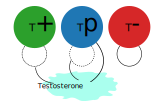
\includegraphics[width=\textwidth]{schematic}
        \caption{Schematic representation of cell types}
      \end{figure}}
    \end{column}
  \end{columns}
  \onslide<3->{\begin{table}
    \centering
    \begin{tabular}{|l|c|c|c|c|}
    \hline
    Cell type & \parbox[t]{1.8cm}{Testosterone\\dependent} & \parbox[t]{1.8cm}{Testosterone\\producing} & Mechanism of resistance\\
    \hline
    $T^+$ & Yes & No & N/A \\
    $T^p$ & Yes & Yes & Cholesterol $\xrightarrow{CYP17\alpha}$ Testosterone \\
    $T^-$ & No & No & AR\footnotemark[1] mutation\\
    \hline
    \end{tabular}
  \end{table}}
  \footnotetext[1]{AR: Androgen Receptors}
\end{frame}

\section{How do we model this?}
\begin{frame}{System of equations}
  \begin{columns}
    \begin{column}{0.55\textwidth}
      \onslide<1->{\begin{equation}
        \frac{dy_i}{dt} = r_i y_i (1 - \frac{\sum_j y_j}{1 + K_{i,max} f_i(O_2) f_i(test)} )- \delta_i y_i
        \label{celleq}
      \end{equation}}
      \onslide<2->{\begin{equation}
        f_i(res) = \begin{cases}
          1 &\text{if } ul_{res,i} \leq res\\
          \frac{res-ll_{res,i}}{ul_{res,i}-ll_{res,i}} &\text{if } ll_{res,i} < res < ul_{res,i}\\
          0 &\text{if } res \leq ll_{res,i}\\
        \end{cases}
        \label{freseq}
      \end{equation}}
      \onslide<3->{\begin{equation}
        \frac{dO_2}{dt} = p_{O_2} - \sum_i \mu_{O_2,i} y_i - \lambda_{O_2} O_2
        \label{o2eq}
      \end{equation}
      \begin{equation}
        \frac{d(test)}{dt} = p_{test} y_{T^p} - \sum_i \mu_{test,i} y_i - \lambda_{test} test
        \label{testeq}
      \end{equation}}
    \end{column}
    \begin{column}{0.45\textwidth}
      \onslide<2->{\begin{figure}[h]
        \centering
        \includegraphics[width=\textwidth]{f_res}
        \caption{Function dependence of carrying capacity on resource}
      \end{figure}}
      \onslide<4->{\begin{itemize}
        \item Assumptions: No mutation, no spatial structure, well mixed
        \item Defined $\mathbb{R}_{\geq 0}$, $y_i < 1 =$ extinction
      \end{itemize}}
    \end{column}
  \end{columns}
  \footnotetext[1]{$i \in \{T^+,T^p,T^-\}$, $res \in \{O_2,test\}$}
  \footnotetext[2]{$ll$: lower limit, $ul$: upper limit}
\end{frame}

\begin{frame}{Parameters Used}
\begin{itemize}
  \item<1-> Some values directly from literature based on cell line data \cite{Jain, HailJr}
  \begin{itemize}
    \item $T^+$: LNCaP
    \item $T^p$: 22Rv1
    \item $T^-$: PC3
  \end{itemize}
  \item<2-> Some values derieved from literature via contraint equations \cite{atcc, Steward, Titus}
  \item<3-> Study Parameters:
    \begin{itemize}
      \item Resource limitations: varied using lower and upper limits
      \item Initial seeding: different ratios of cell types and total population
    \end{itemize}
\end{itemize}

\end{frame}
